\documentclass[12pt,a4paper]{book} % article, report, book.
%%%%%%%%%%%%%%%%%%%%%%%%%%%%%%%%%%%%%%%%%%%%%%%%%%%%%%%%%%%%%%%%%%%
%%% Documento LaTeX                                             %%%
%%%%%%%%%%%%%%%%%%%%%%%%%%%%%%%%%%%%%%%%%%%%%%%%%%%%%%%%%%%%%%%%%%%
% Título: Paquetes
% Autor:  Ignacio Moreno Doblas
% Fecha:  2014-02-01
%%%%%%%%%%%%%%%%%%%%%%%%%%%%%%%%%%%%%%%%%%%%%%%%%%%%%%%%%%%%%%%%%%%
% Tabla de materias:
% 1 Codificación e idioma %
% 2 Matemáticas y Física %
% 3 Gráficos%
% 4 Estilo y formato%
%%%%%%%%%%%%%%%%%%%%%%%%%%%%%%%%%%%%%%%%%%%%%%%%%%%%%%%%%%%%%%%%%%%

%1 Codificación e idioma%
\usepackage[utf8]{inputenc} %Codificación en utf8%
\usepackage[spanish]{babel} %Hyphenation (Guionado) en español%
\usepackage[T1]{fontenc} %Codificación de fuente%
\usepackage{eurofont} %Tipografía euro (€)%

%2 Matemáticas y Física %
% Importante para ecuaciones, magnitudes y unidades%
\usepackage{amssymb,amsmath,latexsym,amsfonts} % paquetes estándar%
\usepackage[squaren]{SIunits} %Paquete para magnitudes y unidades físicas%
\usepackage{ifthen} %sentencias if y while%

%3 Gráficos%
\usepackage{graphics,graphicx} %paquetes gráficos estándar%
\usepackage{wrapfig} %paquete para gráfica lateral%
\usepackage[rflt]{floatflt} %figuras flotantes%
  % \begin{floatingfigure}[r]/[l]{4.5cm}
  % \end{floatingfigure}
\usepackage{graphpap} %comando \graphpaper en el entorno picture%

%4 Estilo y formato%
\usepackage{fancyhdr} %cabeceras y pies mejor que con \pagestyle{}%
\usepackage{titlesec,titletoc} %Formateo de secciones y títulos%
\raggedbottom %Para fragmentar versos en varias páginas%
\usepackage{makeidx} %MakeIndex%
%\usepackage{showidx} % Hace que cada comando \index se imprima en la página donde se ha puesto (útil para corregir los índices)
\usepackage{alltt} % Define el environment alltt, como verbatim, excepto que \, { y } tienen su significado normal. Se describe en el fichero alltt.dtx.
\usepackage[pdftex,bookmarksnumbered,hidelinks]{hyperref} %hyper-references%
\usepackage{minitoc} % Para poner tablas de contenido en cada capítulo.
\usepackage{listings} % Para escribir piezas de código C, Python, etc. %
%listings configuration
\lstset{
  language=[ARM]Assembler, %Puede ser C, C++, Java, etc.
  showstringspaces=false,
  formfeed=\newpage,
  tabsize=4,
  commentstyle=\itshape,
  basicstyle=\ttfamily,
  morekeywords={models, lambda, forms}
}

\usepackage{tipa} % tipografía IPA (International Phonetic Alphabet)
\usepackage{longtable} %Entorno Longtable, fracciona tablas a lo largo de páginas%
\usepackage{colortbl}
\usepackage{acronym}  %Para expandir automáticamente los acrónimos

%%%%%%%%%%%%%%%%%%%%%%%%%%%%%%%%%%%%%%%%%%%%%%%%%%%%%%%%%%%%%%%%%%%
% Tabla de materias:
% 1 Información del Documento %
% 2 Comandos a nivel de texto %
% 3 Comandos a nivel de entorno %
% 4 Comandos a nivel de página y sección %
% 5 Otros comandos %
%%%%%%%%%%%%%%%%%%%%%%%%%%%%%%%%%%%%%%%%%%%%%%%%%%%%%%%%%%%%%%%%%%%

% 1 Información del Documento %
\newcommand{\pfctitlename}{Guiones de prácticas sobre la plataforma Raspberry Pi}
\newcommand{\pfcauthorname}{Antonio José Villena Godoy}
\newcommand{\pfctutorname}{Rafael Asenjo Plaza \\ Francisco Javier Corbera Peña}
\newcommand{\pfcanno}{2015}

% 2 Comandos a nivel de texto %
\newcommand{\R}{\textsuperscript{\textregistered}}  %Símbolo registrado%
\newcommand{\C}{\textsuperscript{\copyright}} %Símbolo Copyright%
\newcommand{\TM}{\texttrademark} %Símbolo Trade Mark (marca comercial)%

% 2.1 Comandos abreviatura %
\newcommand{\tit}{\textit} %Fuente cursiva (itálica)%
\newcommand{\tbf}{\textbf} %Fuente negrita%
\newcommand{\ttw}[1]{\texttt{#1}} %Fuente máquina de escribir (typewriter)%
%Combinación%
\newcommand{\textittt}[1]{\textit{\texttt{#1}}} %itálica y typewriter%
\newcommand{\textittw}{\textittt} % Otra forma de escribirlo.
\newcommand{\tittw}{\textittw} %Shortened%
\newcommand{\tbftw}[1]{\tbf{\ttw{#1}}}

%Crea una nueva línea y la indenta sin crear interlineado extra.
\newcommand{\nli}{\\ \indent} 

%Para escribir un correo electrónico%
\newcommand{\mailto}[1]{\href{mailto:#1}{#1}}

% Si vas a hacer un uso básico de \index (entradas en el índice de sólo un nivel, sin formatos especiales, etc.), define la orden
\newcommand{\miindex}[1]{#1\index{#1}}

\newcommand{\hs}{\hspace} % Abreviatura espacio horizontal
\newcommand{\vs}{\vspace} % Abreviatura espacio vertical

% Abreviaturas para los conjuntos de números más comunes.
\newcommand{\realnumbers}{\mathbb R}
\newcommand{\naturalnumbers}{\mathbb N}
\newcommand{\integernumbers}{\mathbb Z}
\newcommand{\rationalnumbers}{\mathbb Q}
\newcommand{\complexnumbers}{\mathbb R}
\newcommand{\irrationalnumbers}{\mathbb I}

% Doble barra sobre una letra (para expresar las matrices).
\newcommand{\doublebar}[1]{\bar{\bar{#1}}} 
% Ej: \vector(y) = \doublebar(A) \vector(x) (Stma. lineal de ec.)

% 3 Comandos a nivel de entorno %
\newcommand{\benu}{\begin{enu}} % Begin enumerate
\newcommand{\eenu}{\end{enu}}   % End enumeration

%Comando para escribir código Python
\newcommand{\code}[3]{
  %\hrulefill
  %\subsection*{#1}
  %\subsubsection{#1}
  \lstinputlisting{#2}
  %#1\\
  \begin{table}[h!]
    \centering
    \caption{#1}
    \label{#3}
  \end{table}
  \vspace{2em}
}

% 4 Comandos a nivel de página y sección %
%Crea página en blanco
\newcommand{\blankpage}{\clearpage{\pagestyle{empty}\cleardoublepage}}

% Versión x del comando section: sin numeración pero sí aparece en la tabla de contenidos.
\newcommand{\sectionx}[1]{
  \section*{#1}
  \addcontentsline{toc}{section}{#1}
}

% Versión y del comando section: sin numeración y NO aparece en la tabla de contenidos.
\newcommand{\sectiony}[1]{
  \section*{#1}
}

% Versión x del comando chapter: sin numeración pero sí  aparece en la tabla de contenidos.
\newcommand{\chapterx}[1]{
  \chapter*{#1}
  %\addcontentsline{toc}{chapter}{#1} %Caused by minitoc package%
  \addstarredchapter{#1} %For minitoc package%
}

% substituto del comando \chapter: incluye estilo de página.
\newcommand{\chapterbegin}[1]%
  {%
    \pagestyle{fancy}
    \fancyhead[LE,RO]{\thepage}
    \fancyhead[LO]{Capítulo \thechapter. #1}
    %\fancyhead[RE]{Parte \thepart \rightmark} %
    \fancyhead[RE]{\nouppercase{\rightmark}} %
        
    \chapter{#1}
  }

% Versión x del comando \chapterbegin: sin numeración y aparece en la tabla de contenidos.
\newcommand{\chapterbeginx}[1]%
  {%
    \pagestyle{fancy}
    \fancyhead[RO,LE]{\thepage}
    \fancyhead[RE,LO]{#1}
    %\fancyhead[LO]{Chapter \thechapter}
    %\fancyhead[RE]{Part \thepart} %
    
    \chapterx{#1}
  }

%Fin de capítulo
\newcommand{\chapterend}{\pagestyle{empty}\cleardoublepage \thispagestyle{empty}}
%Si fuera un artículo en lugar un libro, \clearpage en lugar de \cleardoublepage

% 5 Otros comandos %
%\let\Oldpart\part
%\newcommand{\parttitle}{}
%\renewcommand{part}[1]{\Oldpart{#1}\renewcommand{\parttitle}{#1}} %Header customization%

%Cambiar el título índice de capítulo a ``Contenido''.
\renewcommand{\mtctitle}{Contenido}

\dominitoc % Para tablas de contenidos por capítulo.

\addto{\captionsspanish}{
  \renewcommand{\listtablename}{Índice de Tablas}
  \renewcommand{\tablename}{Tabla} } % Por ejemplo, modificar el nombre de 'Cuadro' a 'Tabla'.

\addto{\captionsspanish}{
  \renewcommand{\contentsname}{Índice} }

%Si se desea cambiar el tipo de letra a Arial
% por cualquier razón, descomentar las siguientes
% dos líneas
%\renewcommand{\rmdefault}{phv} % Arial
%\renewcommand{\sfdefault}{phv} % Arial
  
%\addto{\captionsspanish}{
% \renewcommand{\partname}{Fase} }

%\addto{\captionsspanish}{%
%    \renewcommand{\refname}{\vspace{-4.5ex}}} % Para que no aparezca el texto 'referencias' en la bibliografía.

% Modifica el interlineado
%\renewcommand{\baselinestretch}{1.5}

   \definecolor{myfboxbg}{gray}{0.9}
   \newsavebox{\efcaja}
   \newenvironment{myfbox}{\begin{lrbox}{\efcaja}}
               {\end{lrbox}{\colorbox{myfboxbg}{\usebox{\efcaja}}}}

%%%%%%%%%%%%%%%%%%%%%%%%%%%%%%%%%%%%%%%%%%%%%%%%%%%%%%%%%%%%%%%%%%%
% Tabla de materias:
%--------------------%
% 1 dobleindent
% 2 izqindent
% 3 dobleindentx
% 4 ite
% 5 descript
% 6 enu
% 7 itemization
% 8 sinopsis
% 9 objetivo
%%%%%%%%%%%%%%%%%%%%%%%
% Para conocer los parámetros de diseño de las listas, tales como
%  los márgenes izquierdo, derechos y los diferentes saltos,
%  véase el archivo ``List layout.png'' que acompaña esta plantilla.
% Así se conocerá mejor cómo adaptar un entorno según los requisitos 
%  del usuario.

%%%%%%%%%%%%%%%%%%%%%%%
% Definición de longitudes para usar en los entornos:
%
% Normal parskip.
\newlength{\parskipenv}
\setlength{\parskipenv}{\parskip}

\newlength{\parindentenv}
\setlength{\parindentenv}{\parindent}
%%%%%%%%%%%%%%%%%%%%%%%

% 1 dobleindent
%El entorno dobleindent está pensando para escribir párrafos con doble indentación a cada lado.
%Tiene dos parámetros de entrada con las distancias medidas desde los márgenes de página.

\newenvironment{dobleindent}[2]
  %Comienzo de nuevo entorno%
  {
  \begin{list}
    {}
    {
    % Left and right margins:
    \leftmargin = #1 
    \rightmargin = #2
    %
    % Separation from preceding and following text:
    \topsep = 0ex
    \partopsep = 0ex
    \parsep = \parskipenv
    %
    % Indentation for paragraphs:
    \itemsep = \parskipenv
    \itemindent = \parindentenv
    \listparindent = \itemindent
    %
    % Horizontal separation from label:
    \labelsep = 1ex
    \settowidth{\labelwidth}{0cm}
    }
    
     \item}
  % End new env
  {\end{list}}

%%%%%%%%%%%%%%%%%%%%%%%%%%%%%
%2 izqindent
% El entorno izqindent sólo crea un párrafo indentado a la izquierda.
\newenvironment{izqindent}[1]
{
\begin{dobleindent}{#1}{0cm}
}
{
\end{dobleindent}
}

%%%%%%%%%%%%%%%%%%%%%%%%%%%%%
% 3 dobleindentx
% El entorno dobleindentx es una variación del dobleindent usando leftskip y rightskip.
% Aunque es más limitado, también se puede usar.
\newenvironment{dobleindentx}[2] % Sólo funciona en modo paragraph
{ % Preamble
  \leftskip = #1
  \rightskip = #2
}
{ % Postamble
\leftskip = 0cm
\rightskip = 0cm
}

%%%%%%%%%%%%%%%%%%%%%%%%%%%%%
% 4 ite
% El entorno ite es una modificación del entorno itemize estándar de \LaTeX. Puede usarse o modificarse si el usuario lo desea.
% También puede parametrizarse el entorno enumerate o description de forma equivalente.
\newenvironment{ite}
  {
    \begin{izqindent}{\parindent}
    \hspace{-\parindent}  % compensación del sangrado que introduce el entorno.
    \vspace{-1.0\parskip} % compensación del \parskip que introduce el entorno.
    \vspace{-\baselineskip} % compensación por la línea que introduce el entorno.
    \begin{itemize}
  }
  {
    \end{itemize}
    \end{izqindent}
  }

%%%%%%%%%%%%%%%%%%%%%5
% commando stdformat para formatear los entornos descript, enu y itemization.
\newcommand{\stdformat}
  {% Declarations for format presentation.
    %     
    % Separation from preceding and following text:
    \setlength{\topsep}{0ex}%
    \setlength{\partopsep}{0ex} %
    %
    % Horizontal separation from label:
    \labelsep = 1ex
    \setlength{\labelwidth}{0ex}
    %
    % Left and right margins: 
    \setlength{\leftmargin}{1cm}%
    \addtolength{\leftmargin}{\labelsep}
    \setlength{\rightmargin}{0ex}
    %  
    % Indentation for paragraphs:
    \setlength{\itemindent}{-\leftmargin}%
    \addtolength{\itemindent}{1ex}
    \setlength{\listparindent}{\parindent}%
    %   
    % Separation between paragraphs.
    \setlength{\parsep}{\parskipenv}% 
    \setlength{\itemsep}{1ex}
  }

%%%%%%%%%%%%%%%%%%%%%%%%%%%%%
% 5 descript

\newenvironment{descript}
  % Beginning new env def.
  {
    \begin{list}
      {} % No default label for \item.
      {
        % Declarations for format presentation.
        \stdformat
        %
        \renewcommand{\makelabel}[1]{\normalfont\bfseries##1\hfil}
      }
  }
  % Ending new env def.
  {
    \hspace*{\fill} \\ \end{list}
  } % Se introduce un salto de línea para que el texto siguiente esté separado.
%END newenvironment{descript}

%%%%%%%%%%%%%%%%%%%%%%%%%%%%%
% 6 enu
\newcounter{itemnumber} % Counter for the environment.

\newenvironment{enu}
  % Beginning new env def.
  {
    \begin{list}
    {
      \raggedleft \arabic{itemnumber}
    }
    {
      \usecounter{itemnumber}
      \stdformat
    }
  }
  {
    \end{list}
  }

%%%%%%%%%%%%%%%%%%%%%%%%%%%%%
% 7 itemization
\newenvironment{itemization}
  % Beginning new env def.
  {
    \begin{list}
      {$\bullet$} % No default label for \item.
      {
        % Declarations for format presentation.
        \stdformat
      }
  }
  % Ending new env def.
  {
    \end{list}
  }


%%%%%%%%%%%%%%%%%%%%%%%%%%%%%
% 8 sinopsis
\newenvironment{sinopsis}{%[1]{
  \sectiony{Sinopsis}
  %\label{#1}
} {
  \pagebreak
}

%%%%%%%%%%%%%%%%%%%%%%%%%%%%%
% 9 objetivo
\newenvironment{objetivo}{%[1]{
  \sectiony{Objetivo}
  %\label{#1}
} {
}

%%%%%%%%%%%%%%%%%%%%%%%%%%%%%%%%%%%%%%%%%%%%%%%%%%%%%%%%%%%%%%%%%%%
% Tabla de materias:
%--------------------%
% 1 Márgenes de página
%%%%%%%%%%%%%%%%%%%%%%%
% Para conocer los parámetros de diseño de páginas, tales como
%  los márgenes izquierdo, derecho, anchura de página, etc.
%  véase el archivo ``Page layout.png'' que acompaña esta plantilla.
% Así se conocerá mejor cómo adaptar el documento según los 
%  requisitos del usuario.

% 1 Márgenes de página
%-------------------------------%
% Parámetros de estilo de página.
% DIN A4: 29.7 cm x 21 cm
%   área neta: 3 cm + 3 cm + 15 cm.
%
% Definición de márgenes de página
%  even para páginas pares
%  odd  para páginas impares
\newlength{\realoddsidemargin}    % \oddsidemargin menos 1 in.
\newlength{\realevensidemargin}   % \evensidemargin menos 1 in.
\newlength{\realtopmargin}        % \topmargin menos 1 in.
%
% Asignación de márgenes de página
% ASIGNESE en caso de querer cambiarlo
\setlength{\realtopmargin}{2cm}     % REAL top margin.
\setlength{\realoddsidemargin}{3cm}   % REAL oddside margin.
\setlength{\realevensidemargin}{3cm}  % REAL evenside margin.
\setlength{\hoffset}{0cm}
\setlength{\voffset}{0cm}
%
% Substracción de 1 pulgada de compensación
%  (véase ``Page Layout.png'' para más información)
\addtolength{\realoddsidemargin}{-1in}  % 1 inch = 2.54 cm.
\addtolength{\realevensidemargin}{-1in}
\addtolength{\realtopmargin}{-1in}
%
% Asignación de anchuras y márgenes
% No hay notas al margen
\setlength{\marginparsep}{0cm} % No van a existir notas al margen
\setlength{\marginparwidth}{0cm} % No van a existir notas al margen
%
% Asignación de anchura de texto
\setlength{\textwidth}{15cm}  % Anchura neta del texto (globalmente).
%
% Asignación de márgenes par, impar y en altura
\setlength{\oddsidemargin}{\realoddsidemargin}  % odd-page left margin (global).
\setlength{\evensidemargin}{\realoddsidemargin} % even-page left margin (global).
\setlength{\topmargin}{\realtopmargin}          % top margin (Global).

% Se puede usar también el paquete chngpage.

%%%%%%%%%%%%%%%%%%%%%%%%%%%%%%%%%%%%%%%%%%%%%%%%%%%%%%%%%%%%%%%%%%
%   1 Length commands.          %
%-------------------------------%
% Defines new length command (e.g., \newlength{\gnat}}
% \newlength{}
%
% Set lenght to a value.
% \setlength{\gnat}{length}
% \addtolength{}{}
%
% Sets the value of a length command equal to the width of a specified piece of text; e.g., \settowidth{\parindent}{\em small}.
% \settowidth{}{}
% Set the value of a height. e.g., \settoheight{\parskip}{Gnu}
% \settoheight{}{}
% Set the value that extends below the line. e.g., \settodepth{\parskip}{gnu}.
% \settodepth{}{}
%
% To multiply a length, write: 7.0\gnat = \gnat * 7.0
%%%%%%%%%%%%%%%%%%%%%%%%%%%%%%%%%%%%%%%%%%%%%%%%%%%%%%%%%%%%%%%%%%

\begin{document}

%%%%%%%%%%%%%%%%%%%%%%%%%%%%%%%%%%%%%%%%%%%%%%%%%%%%%%%%%%%%%%

\chapterbegin{E/S a bajo nivel}
\label{chp:Subrut}
\minitoc

{\bf Objetivos}: Hasta ahora hemos programado en ensamblador sobre
la capa que nos ofrece el sistema operativo. Nosotros llamamos a una
función y ésta hace todo lo demás: le dice al sistema operativo lo
que tiene que hacer con tal periférico y el sistema operativo (en concreto
el kernel) le envía las órdenes directamente al periférico, al espacio
de memoria donde esté mapeado el mismo.

Lo que vamos a hacer en este capítulo es comunicarnos directamente con los
periféricos, para lo cual debemos prescindir totalmente del sistema operativo.
Este modo de acceder directamente al hardware de la máquina se denomina {\tt Bare Metal},
que traducido viene a ser algo como {\tt Metal desnudo}, haciendo referencia a
que estamos ante la máquina tal y cómo es, sin ninguna capa de abstracción de
por medio.

Veremos ejemplos de acceso directo a periféricos, en concreto al LED de la placa
auxiliar y a los temporizadores, que son bastante sencillos de manejar.

\section{Lectura previa}

\subsection{Librerías y Kernel, las dos capas que queremos saltarnos}

Anteriormente hemos utilizado funciones específicas para
comunicarnos con los periféricos. Si por ejemplo necesitamos escribir
en pantalla, llamamos a la función {\tt printf}. Pues bien, entre
la llamada a la función y lo que vemos en pantalla hay 2 capas de por medio.

Una primera capa se encuentra en la librería runtime que acompaña al
ejecutable, la cual incluye sólamente el fragmento de código de la
función que necesitemos, en este caso en {\tt printf}. El resto de
funciones de la librería ({\tt stdio}), si no las invocamos no aparecen
en el ejecutable. El enlazador se encarga de todo esto, tanto de ubicar
las funciones que llamemos desde ensamblador, como de poner la dirección
numérica correcta que corresponda en la instrucción {\tt bl printf}.

Este fragmento de código perteneciente a la primera capa sí que podemos
depurarlo mediante {\tt gdb}. Lo que hace es, a parte del formateo que
realiza la propia función, trasladar al sistema operativo una determinada
cadena para que éste lo muestre por pantalla. Es una especie de traductor
intermedio que nos facilita las cosas. Nosotros desde ensamblador también
podemos hacer llamadas al sistema directamente como veremos posteriormente.

La segunda capa va desde que hacemos la llamada al sistema hasta que se
produce la transferencia de datos al periférico, retornando desde la llamada
al sistema y volviendo a la primera capa, que a su vez retornará el control
a la llamada a librería que hicimos en nuestro programa inicialmente.

En esta segunda capa se ejecuta código del kernel, el cual no podemos depurar.
Además el procesador entra en un modo privilegiado, ya que en modo usuario (el
que se ejecuta en nuestro programa ensamblador y dentro de la librería) no
tenemos privilegios suficientes como para acceder a la zona de memoria que
mapea los periféricos.

En la figura \ref{fig:capas} podemos ver el código llamador junto con las dos
capas.

\begin{figure}[h]
  \centering
    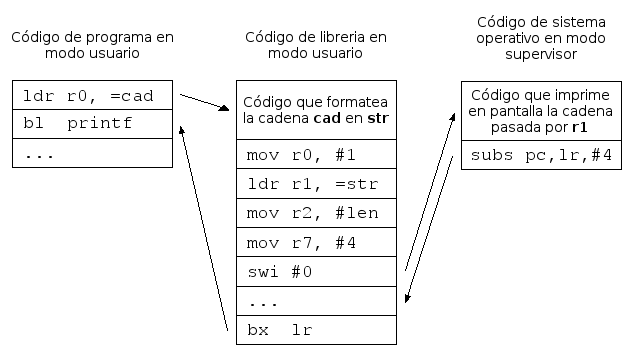
\includegraphics[width=14cm]{graphs/capas.png}
  \caption{Funcionamiento de una llamada a printf}
  \label{fig:capas}
\end{figure}

Ahora veremos un ejemplo en el cual nos saltamos la capa intermedia para
comunicarnos directamente con el kernel vía llamada al sistema. En este ejemplo
vamos a escribir una simple cadena por pantalla, en concreto "Hola Mundo!".

\begin{lstlisting}[caption={esbn1.s},label={lst:codigoPract4_1},escapeinside={@}{@}]
.data

cadena: .asciz "Hola Mundo!\n"
cadenafin:

.text
.global main
 
main:   push    {r7, lr}           /* preservamos reg.*/
        mov     r0, #1             /* salida estándar */
        ldr     r1, =cadena        /* cadena a enviar */
        mov     r2, #cadenafin-cadena     /* longitud */
        mov     r7, #4             /* seleccionamos la*/
        swi     #0        /* llamada a sistema 'write'*/
        mov     r0, #0             /* devolvemos ok   */
        pop     {r7, lr}           /* recuperamos reg.*/
        bx      lr                 /* salimos de main */
\end{lstlisting}

La instrucción que ejecuta la llamada al sistema es {\tt swi \#0},
siempre tendrá cero como valor inmediato. El código numérico de
la llamada y el número de parámetros podemos buscarlo en cualquier
manual de Linux, buscando ``Linux system call table'' en Google. En
nuestro caso la llamada {\tt write} se corresponde con el código
4 y acepta tres parámetros: manejador de fichero, dirección de
los datos a escribir (nuestra cadena) y longitud de los datos.

En general se tiende a usar una lista reducida de posibles llamadas
a sistema, y que éstas sean lo más polivalentes posibles. En este
caso vemos que no existe una función específica para escribir en
pantalla. Lo que hacemos es escribir bytes en un fichero, pero usando
un manejador especial conocido como salida estándar, con lo cual todo
lo que escribamos a este fichero especial aparecerá por pantalla.

Pero el propósito de este capítulo no es saltarnos una capa
para comunicarnos directamente con el sistema operativo. Lo que queremos
es saltarnos las dos capas y enviarle órdenes directamente a los periféricos.
Para esto tenemos prescindir del sistema operativo, o lo que es lo mismo,
hacer nosotros de sistema operativo para realizar las tareas que queramos.

Este modo de trabajar (como hemos adelantado) se denomina Bare Metal, porque
accedemos a las entrañas del hardware. En él podemos hacer desde cosas
muy sencillas como encender un LED hasta programar desde cero nuestro propio
sistema operativo.

\subsection{Ejecutar código en Bare Metal}

El ciclo de ensamblado y enlazado es distinto en un programa Bare Metal. Hasta
ahora hemos creado ejecutables, que tienen una estructura más compleja, con cabecera y
distintas secciones en formato {\tt ELF}. Toda esta información le viene muy bien al
sistema operativo, pero en un entorno Bare Metal no disponemos de él. Lo que se carga
en {\tt kernel.img} es un binario sencillo, sin cabecera, que contiene directamente
el código máquina de nuestro programa y que se cargará en la dirección de RAM {\tt 0x8000}.

Lo que para un ejecutable hacíamos con esta secuencia.
\begin{lstlisting}
        as -o ejemplo.o ejemplo.s
        gcc -o ejemplo ejemplo.o
\end{lstlisting}

En caso de un programa Bare Metal tenemos que cambiarla por esta otra.
\begin{lstlisting}
        as -o ejemplo.o ejemplo.s
        ld -e 0 -Ttext=0x8000 -o ejemplo.elf ejemplo.o
        objcopy ejemplo.elf -O binary kernel.img
\end{lstlisting}

Otra característica de Bare Metal es que sólo tenemos una sección de código (la sección
.text), y no estamos obligados a crear la función
{\tt main}. Al no ejecutar ninguna función no tenemos la posibilidad de salir del
programa con {\tt bx lr}, al fin y al cabo no hay ningún sistema operativo detrás al
que regresar. Nuestro programa debe trabajar en bucle cerrado. En caso de tener una
tarea simple que querramos terminar, es preferible dejar el sistema colgado con un
bucle infinito como última instrucción.

El proceso de arranque de la Raspberry Pi es el siguiente:

\begin{itemize}
  \item Cuando la encendemos, el núcleo ARM está desactivado. Lo primero que se activa es el
        núcleo GPU, que es un procesador totalmente distinto e independiente al ARM. En este
        momento la SDRAM está desactivada.
  \item El procesador GPU empieza a ejecutar la primera etapa del bootloader (son 3 etapas), que
        está almacenada en ROM dentro del mismo chip que comparten ARM y GPU. Esta primera etapa
        accede a la tarjeta SD y lee el fichero {\tt bootcode.bin} en caché L2 y lo ejecuta,
        siendo el código de {\tt bootcode.bin} la segunda etapa del bootloader.
  \item En la segunda etapa se activa la SDRAM y se carga la tercera parte del bootloader, cuyo
        código está repartido entre {\tt loader.bin} (opcional) y {\tt start.elf}.
  \item En tercera y última etapa del bootloader se accede opcionalmente a dos archivos ASCII de
        configuración llamados {\tt config.txt} y {\tt cmdline.txt}. Lo más relevante de esta
        etapa es que cargamos en RAM (en concreto en la dirección 0x8000) el archivo
        {\tt kernel.img} con código ARM, para luego ejecutarlo y acabar con el bootloader, pasando
        el control desde la GPU hacia la CPU.
        Este último archivo es el que nos interesa modificar para nuestros propósitos, ya que es
        lo primero que la CPU ejecuta y lo hace en modo privilegiado, es decir, con acceso total
        al hardware.
\end{itemize}

De todos estos archivos los obligatorios son {\tt bootcode.bin}, {\tt start.elf} y
{\tt kernel.img}. Los dos primeros los bajamos del repositorio oficial
\footnote{\url{https://github.com/raspberrypi}} y el tercero {\tt kernel.img} es el que nosotros
vamos a generar. Estos tres archivos deben estar en el directorio raíz de la primera partición
de la tarjeta SD, la cual debe estar formateada en FAT32.

El proceso completo que debemos repetir cada vez que desarrollemos un programa nuevo
en Bare Metal es el siguiente:

\begin{itemize}
  \item Apagamos la Raspberry.
  \item Extraemos la tarjeta SD.
  \item Introducimos la SD en el lector de nuestro ordenador de desarrollo.
  \item Montamos la unidad y copiamos (sobreescribimos) el kernel.img que acabamos
        de desarrollar.
  \item Desmontamos y extraemos la SD.
  \item Insertamos de nuevo la SD en la Raspberry y la encendemos.
\end{itemize}

Es un proceso sencillo para las prácticas que vamos a hacer, pero para proyectos más largos
se vuelve bastante pesado de realizar. Hay varias alternativas que agilizan el ciclo de
trabajo, donde no es necesario extraer la SD y por tanto podemos actualizar el {\tt kernel.img}
en cuestión de segundos.

\begin{itemize}
  \item Cable JTAG con software Openocd \footnote{\url{http://openocd.sourceforge.net}}
  \item Cable USB-serie desde el ordenador de desarrollo hacia la Raspberry, requiere
        tener instaladas las herramientas de compilación cruzada en el ordenador de desarrollo.
  \item Cable serie-serie que comunica dos Raspberries, una orientada a desarrollo y la otra
        para ejecutar los programas en Bare Metal. No es imprescindible trabajar directamente
        con la Raspberry de desarrollo, podemos acceder vía ssh con nuestro ordenador habitual,
        sin necesidad de tener instaladas las herramientas de compilación en el mismo.
\end{itemize}

En las dos últimas opciones lo que se almacena en el kernel.img de la SD es un bootloader
que lee continuamente del puerto serie y en el momento en que recibe un archivo lo carga
en RAM y lo ejecuta. El protocolo de transferencia que emplea el bootloader se llama XMODEM,
y los parámetros del puerto serie son: 8 bits de datos, sin paridad, 1 bit de parada, sin
flujo de control y velocidad de transferencia de 115200 baudios. Son todos parámetros por
defecto excepto la velocidad, por lo que hay que asegurarse de cambiar la velocidad antes
de proceder a transferir el archivo en nuestro programa terminal. En Windows tenemos varias
alternativas, como {\tt HyperTerminal} o {\tt Tera Term}. En Linux tenemos utilidades equivalentes
como {\tt minicom}, sin embargo hay una forma de automatizar el proceso en línea de comandos
con el comando {\tt sx}, que es creando el siguiente script {\tt enviar}.

\begin{lstlisting}
stty -F /dev/ttyAMA0 115200
sx $1 < /dev/ttyAMA0 > /dev/ttyAMA0
\end{lstlisting}

Para enviar un archivo con este script, lo único que tenemos que hacer es escribir lo siguiente
bajo línea de comandos.

\begin{lstlisting}
./enviar kernel.img
\end{lstlisting}

Para más información sobre estos métodos recomendamos que sigan los
README del siguiente repositorio \footnote{\url{https://github.com/dwelch67/raspberrypi}}.

\subsection{Acceso a periféricos}

Los periféricos se controlan leyendo y escribiendo datos a los registros asociados. No
confundir estos registros con los registros de la CPU. Un registro asociado a un periférico
es un ente, normalmente del mismo tamaño que el ancho del bus de datos, que sirve para
configurar diferentes aspectos del mismo. No se trata de RAM, por lo que no se garantiza que
al leer de un registro obtengamos el último valor que escribimos. Es más, incluso hay
registros que sólo admiten ser leídos y otros que sólo admiten escrituras. La funcionalidad
de los registros también es muy variable, incluso dentro de un mismo registro los diferentes
bits del mismo tienen distinto comportamiento.

Como cada periférico se controla de una forma diferente, no hay más remedio que leerse
el datasheet del mismo si queremos trabajar con él. En nuestro caso queremos encender un LED
en la placa auxiliar, está conectada al puerto GPIO (entrada/salida de propósito general) y
cuyo conector se encuentra en la esquina superior izquierda de la Raspberry, son dos filas
de 13 pines cada una.

\subsubsection{GPIO}

El datasheet que tenemos que buscar es el siguiente
\footnote{\url{http://www.raspberrypi.org/wp-content/uploads/2012/02/BCM2835-ARM-Peripherals.pdf}},
ya que el dispositivo GPIO se encuentra en el propio chip (el mismo que contiene CPU y GPU).
En el primer capítulo nos encontramos con el siguiente párrafo.

{\it Physical addresses range from 0×20000000 to 0x20FFFFFF for peripherals. The bus addresses
for peripherals are set up to map onto the peripheral bus address range starting at
0x7E000000. Thus a peripheral advertised here at bus address 0x7Ennnnnn is available
at physical address 0x20nnnnnn.}

Esto quiere decir que los registros de los periféricos están mapeados en memoria en
0×20nnnnnn, que es donde haremos las lecturas y escrituras. Pero debemos
trasladar las direcciones que nos indica el datasheet desde 0x7Ennnnnn hasta 0x20nnnnnn,
porque lo primero son direcciones del bus y lo segundo direcciones físicas, y desde
software empleamos estas últimas.

Para nuestros propósitos nos bastaría con acceder a los registros GPFSELx, GPSETx y GPCLRx,
que se corresponden con 13 de los 41 registros que contiene el GPIO. Vemos la tabla con las
direcciones de estos registros (dos de los cuales no se usan, están reservados)

\begin{longtable}{ p{1.8cm} | p{2cm} | p{5cm} | p{1cm} | p{1cm} }
\hline
{\bf Dirección} & {\bf Nombre} & {\bf Descripción} & {\bf Tam.} & {\bf Tipo} \\ \hline
7E200000 & GPFSEL0 & GPIO Function Select 0 & 32 & R/W \\ \hline
7E200004 & GPFSEL1 & GPIO Function Select 1 & 32 & R/W \\ \hline
7E200008 & GPFSEL2 & GPIO Function Select 2 & 32 & R/W \\ \hline
7E20000C & GPFSEL3 & GPIO Function Select 3 & 32 & R/W \\ \hline
7E200010 & GPFSEL4 & GPIO Function Select 4 & 32 & R/W \\ \hline
7E200014 & GPFSEL5 & GPIO Function Select 5 & 32 & R/W \\ \hline
7E200018 & -       & Reservado              & -  & -   \\ \hline
7E20001C & GPSET0  & GPIO Pin Output Set 0  & 32 & W   \\ \hline
7E200020 & GPSET1  & GPIO Pin Output Set 1  & 32 & W   \\ \hline
7E200024 & -       & Reservado              & -  & -   \\ \hline
7E200028 & GPCLR0  & GPIO Pin Output Clear 0 & 32 & W  \\ \hline
7E20002C & GPCLR1  & GPIO Pin Output Clear 1 & 32 & W  \\ \hline
\end{longtable}

Estos registros controlan 54 pines, que a su vez están agrupados
en 6 grupos funcionales de 10 pines cada uno (excepto el último
que es de 4). El LED que queremos controlar se corresponde con el
pin 2 (0 en la revisión 1.0 de la Raspberry) del GPIO, se nombran con
GPIO más el número de pin, en nuestro caso sería GPIO 2 (ó 0). Nótese
que la numeración empieza en 0, desde GPIO 0 hasta GPIO 53. De
todos estos pines sólo diecisiete: 2 (0), 3 (1), 4, 7, 8, 9, 10, 11, 14, 15, 17, 18, 22, 23, 24, 25 y 27 (21).
son accesibles a través del conector, y si disponemos del modelo B+ la lista
aumenta en nueve: 5, 6, 12, 13, 16, 19, 20, 21 y 26.

\begin{figure}[h]
  \centering
    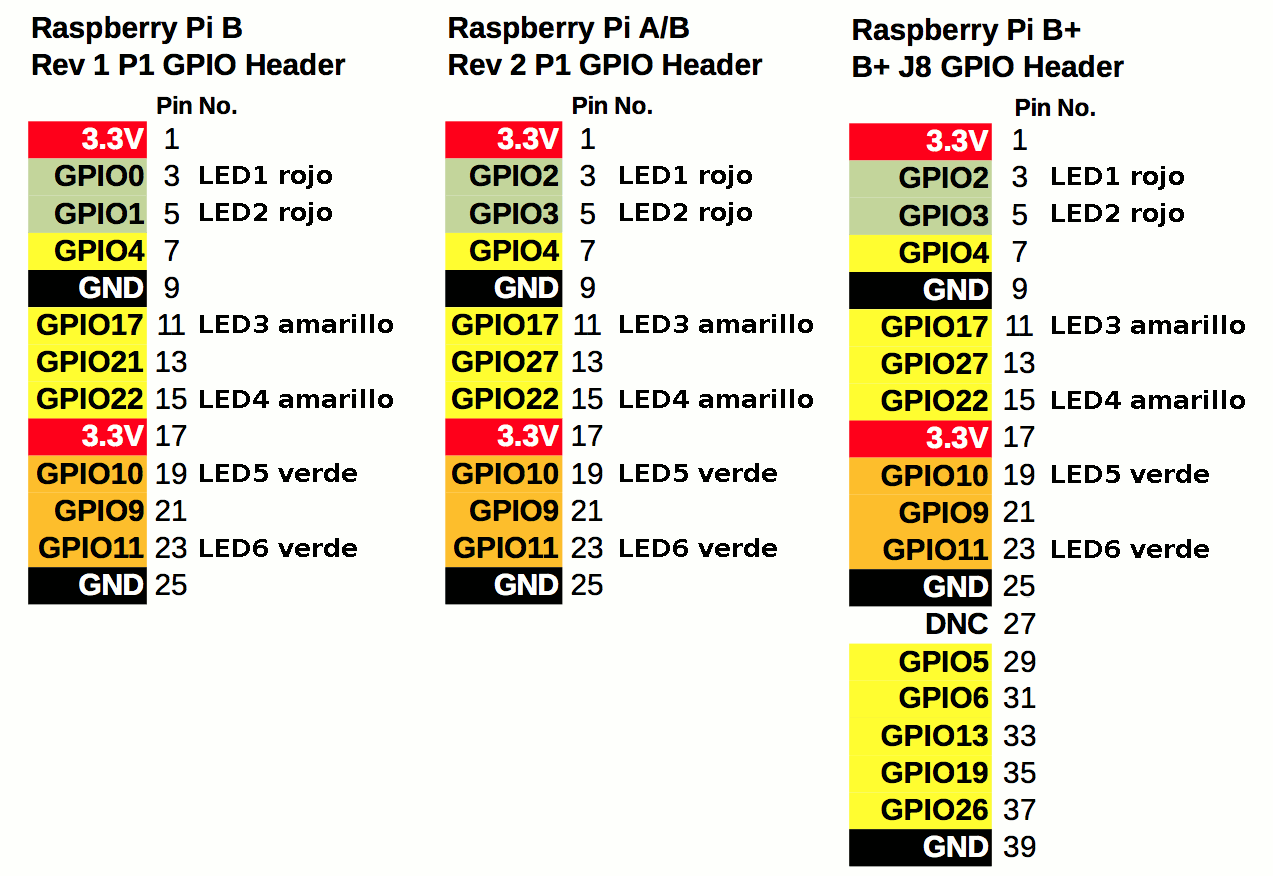
\includegraphics[width=14cm]{graphs/RaspberryGPIOaux.png}
  \caption{Correspondencia LEDs y GPIO}
  \label{fig:pinout}
\end{figure}

Así que la funcionalidad desde GPIO 0 hasta GPIO 9 se controla con
GPFSEL0, desde GPIO 10 hasta GPIO 19 se hace con GPFSEL1 y así
sucesivamente. Nosotros queremos cambiar la funcionalidad de GPIO 2
que está en GPFSEL0, y también lo haremos de GPIO 0 para dar soporte
a las primeras Raspberries. Por defecto cuando arranca la Raspberry
todos los pines están preconfigurados como entradas, y los que se
corresponden con los LEDs rojos además tienen una resistencia de pull-up.
Esto quiere decir que si no hacemos nada los dos LEDs rojos estarán
encendidos. Para evitar esto también configuraremos el segundo LED rojo
como salida, accediendo a los GPIO 1 y 3.

Leyendo más abajo en el datasheet encontramos que
la descripción del registro GPFSEL0 contiene diez grupos funcionales
llamados FSELx (del 0 al 9) de 3 bits cada uno, quedando los dos bits
más altos sin usar. Nos interesa cambiar desde FSEL0 hasta FSEL3, que serían los primeros
12 bits de este registro. Las posibles configuraciones para cada grupo son:

\begin{lstlisting}
000 = GPIO Pin X is an input
001 = GPIO Pin X is an output
100 = GPIO Pin X takes alternate function 0
101 = GPIO Pin X takes alternate function 1
110 = GPIO Pin X takes alternate function 2
111 = GPIO Pin X takes alternate function 3
011 = GPIO Pin X takes alternate function 4
010 = GPIO Pin X takes alternate function 5
\end{lstlisting}

Las funciones alternativas son para dotar a los pines de funcionalidad específicas
como puertos SPI, UART, audio PCM y cosas parecidas. La lista completa
está en la tabla 6-31 (página 102) del datasheet. Nosotros queremos una salida
genérica, nos quedamos con el código {\tt 001}.

Una vez configurado los GPIOs 0/1/2/3 como salida, ya sólo queda saber cómo poner ceros y unos
en los pines GPIOs 0/2, para apagar y encender el primer LED respectivamente (un cero apaga
y un uno enciende el LED).

Para ello tenemos los registros GPSETn y GPCLRn. En principio parece enrevesado el tener
que usar dos registros distintos para escribir en el puerto GPIO, pero no olvidemos que
para ahorrar recursos varios pines están empaquetados en una palabra de 32 bits. Por lo
que si quisiéramos alterar un único pin tendríamos que leer el registro, modificar el bit
en cuestión sin tocar los demás y escribir el resultado de nuevo en el registro. Por suerte
esto no es necesario con registros separados para setear y resetear, tan sólo necesitamos
una escritura en registro poniendo a 1 los bits que queramos setear/resetear y a 0 los bits
que no queramos modificar.

Leemos el datasheet y comprobamos que es así. Además los 54 pines se reparten entre dos
registros GPSET0/GPCLR0 que contine los 32 primeros y en GPSET1/GPCLR1 están los 22
restantes, quedando libres los 10 bits más significativos de GPSET1/GPCLR1. En nuestro
primer ejemplo de Bare Metal sólo vamos a encender el primer LED de la placa auxiliar,
por lo que emplearemos el registro GPCLR0.

\begin{lstlisting}[caption={esbn2.s},label={lst:codigoPract4_2},escapeinside={@}{@}]
        .set    GPBASE,   0x20200000
        .set    GPFSEL0,  0x00
        .set    GPSET0,   0x1c
.text
        ldr     r0, =GPBASE
        ldr     r1, =0b00000000000000000000001001001001
/* guia bits 20..18    xx999888777666555444333222111000*/
        str     r1, [r0, #GPFSEL0]
/* guia bits 16 a 1    10987654321098765432109876543210*/
        mov     r1, #0b00000000000000000000000000000101
        str     r1, [r0, #GPSET0]
infi:   b       infi
\end{lstlisting}

El acceso a los registros lo hemos hecho usando la dirección base donde
están mapeados los periféricos {\tt 0x20200000}. Cargamos esta dirección
base en el registro {\tt r0} y codificamos los accesos a los registros
E/S con direccionamiento a memoria empleando distintas constantes como
desplazamiento en función del registro al que queramos acceder.

Los registros a los que accedemos para encender y apagar el LED vienen indicados
en la figura \ref{fig:gpio1}.

\begin{figure}[h]
  \centering
    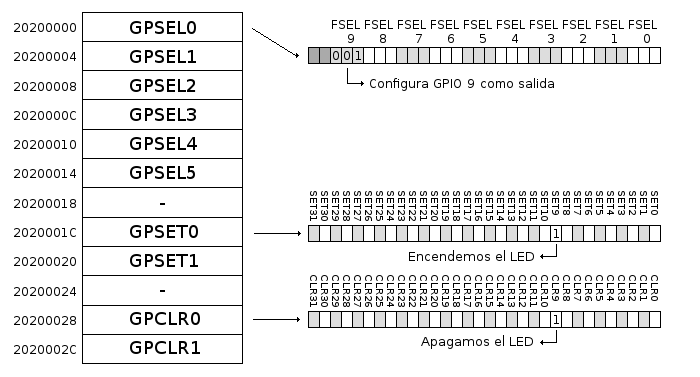
\includegraphics[width=14cm]{graphs/gpio1.png}
  \caption{Registros LED}
  \label{fig:gpio1}
\end{figure}

En realidad sólo se necesita escribir en un bit para encender un LED, la razón de escribir
en dos es para que funcione con distintos modelos de Raspberry. En los 4 LEDs restantes no
existe este problema, cada LED se corresponde con un bit.

El código simplemente escribe dos constantes en dos registros: {\tt GPFSEL0} y {\tt GPSET0}.
Con la primera escritura configuramos 2 LEDs como salida y con la segunda escritura encendemos
el primer LED, para finalmente entrar en un bucle infinito con {\tt infi: b infi}.

Estos son los registros que vamos a usar en este capítulo, pero el dispositivo GPIO tiene
más registros. En la figura \ref{fig:gpio2} tenemos los siguientes.

\begin{figure}[h]
  \centering
    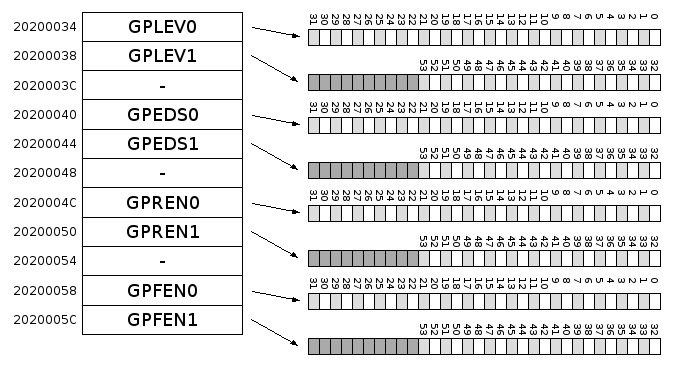
\includegraphics[width=14cm]{graphs/gpio2.png}
  \caption{Otros registros del GPIO}
  \label{fig:gpio2}
\end{figure}

\begin{itemize}
  \item {\tt GPLEVn} Estos registros devuelven el valor del pin respectivo. Si dicho pin está
        en torno a 0V devolverá un cero, si está en torno a 3.3V devolverá un 1.
  \item {\tt GPEDSn} Sirven para detectar qué pin ha provocado una interrupción es caso de
        usarlo como lectura. Al escribir en ellos también podemos notificar que ya hemos procesado
        la interrupción y que por tanto estamos listos para que nos vuelvan a interrumpir sobre
        los pines que indiquemos.
  \item {\tt GPRENn} Con estos registros enmascaramos los pines que queremos que provoquen una
        interrupción en flanco de subida, esto es cuando hay una transición de 0 a 1 en el pin
        de entrada.
  \item {\tt GPFENn} Lo mismo que el anterior pero en flanco de bajada.
\end{itemize}

El resto de registros GPIO están en la figura \ref{fig:gpio3}.

\begin{figure}[h]
  \centering
    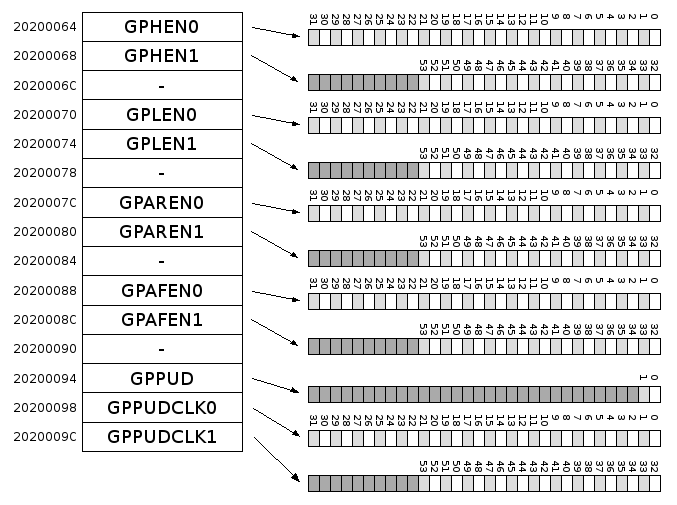
\includegraphics[width=14cm]{graphs/gpio3.png}
  \caption{Otros registros del GPIO}
  \label{fig:gpio3}
\end{figure}

\begin{itemize}
  \item {\tt GPHENn} Enmascaramos los pines que provocarán una interrupción al detectar un
        nivel alto (3.3V) por dicho pin.
  \item {\tt GPLENn} Lo mismo que el anterior pero para un nivel bajo (0V).
  \item {\tt GPARENn y GPAFENn} Tienen funciones idénticas a {\tt GPRENn y GPFENn}, pero permiten
        detectar flancos en pulsos de poca duración.
  \item {\tt GPPUD y GPPUDCLKn} Conectan resistencias de pull-up y de pull-down sobre los pines
        que deseemos. Para más información ver el último ejemplo del siguiente capítulo.
\end{itemize}

\subsubsection{Temporizador del sistema}

Se trata de un reloj que funciona a 1MHz y en cada paso incrementa un contador de 64bits. Nos
viene muy bien para hacer las cuentas porque cada paso del contador se corresponde con un
microsegundo. Los registros asociados al temporizador son los de la figura \ref{fig:systim}.
Básicamente son el contador de 64 bits y cuatro comparadores. El contador está dividido en
dos partes, la parte baja {\tt CLO} y la parte alta {\tt CHI}. La parte alta no nos resulta
interesante, porque tarda poco más de una hora ($2^{32}$ \micro s) en incrementarse y no
va asociado a ningún comparador.

\begin{figure}[h]
  \centering
    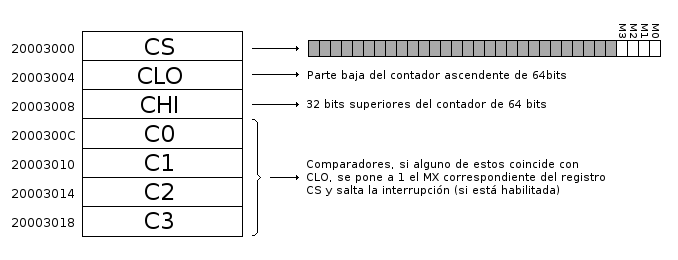
\includegraphics[width=14cm]{graphs/systemtimer.png}
  \caption{System Timer}
  \label{fig:systim}
\end{figure}

Los comparadores son registros que se pueden modificar y se comparan con {\tt CLO}, en el momento
que uno de los 4 comparadores coincida y estén habilitadas las interrupciones para dicho
comparador, se produce una interrupción y se activa el correspondiente bit {\tt Mx}
asociado al registro {\tt CS} (para que en la RTI sepamos qué comparador ha provocado la interrupción).
Los comparadores {\tt C0} y {\tt C2} los emplea la GPU internamente, por lo que nosotros nos
ceñiremos a los comparadores {\tt C1} y {\tt C3}.

Las interrupciones las veremos en la siguiente lección, en los ejemplos de esta sólo vamos
a acceder al registro {\tt CLO} para hacer parpadear al LED a una frecuencia determinada. El
esquema funcional del {\tt System Timer} se muestra en la figura \ref{fig:esqtim}.

\begin{figure}[h]
  \centering
    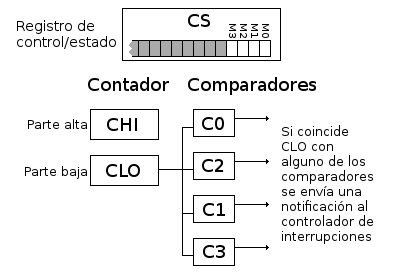
\includegraphics[width=14cm]{graphs/esquematimer.png}
  \caption{Esquema funcional del System Timer}
  \label{fig:esqtim}
\end{figure}


\section{Ejemplos de programas Bare Metal}

\subsection{LED parpadeante con bucle de retardo}

La teoría sobre encender y apagar el LED la sabemos. Lo más sencillo que podemos hacer ahora
es hacer que el LED parpadee continuamente. Vamos a intruducir el siguiente programa en la
Raspberry, antes de probarlo piensa un poco cómo se comportaría el siguiente código.

\begin{lstlisting}[caption={esbn3.s},label={lst:codigoPract4_3}]
        .set    GPBASE,   0x20200000
        .set    GPFSEL0,  0x00
        .set    GPSET0,   0x1c
        .set    GPCLR0,   0x28
.text
        ldr     r0, =GPBASE
/* guia bits 20..18    xx999888777666555444333222111000*/
        ldr     r1, =0b00000000000000000000001001001001
        str     r1, [r0, #GPFSEL0]
/* guia bits 16 a 1    10987654321098765432109876543210*/
bucle:  mov     r1, #0b00000000000000000000000000000101
        str     r1, [r0, #GPSET0]
        mov     r1, #0b00000000000000000000000000000101
        str     r1, [r0, #GPCLR0]
        b       bucle
\end{lstlisting}

Comprobamos que el LED no parpadea sino que está encendido con menos brillo del normal.
En realidad sí que lo hace, sólo que nuestro ojo es demasiado lento como para percibirlo.
Lo siguiente será ajustar la cadencia del parpadeo a un segundo para que podamos observar
el parpadeo. La secuencia sería apagar el LED, esperar medio segundo, encender el LED,
esperar otro medio segundo y repetir el bucle. Sabemos que el procesador de la Raspberry
corre a 700MHz por lo que vamos a suponer que tarde un ciclo de este reloj en ejecutar
cada instrucción. En base a esto vamos a crear dos bucles de retardo uno tras apagar el LED
y otro tras encenderlo de 500ms cada uno. Un bucle de retardo lo único que hace es esperar
tiempo. 

\begin{lstlisting}[caption={Parte de esbn4.s},label={lst:codigoPract4_4}]
.text
        ldr     r0, =GPBASE
        ldr     r1, =0b00000000000000000000001001001001
        str     r1, [r0, #GPFSEL0]
        mov     r1, #0b00000000000000000000000000000101
bucle:  ldr     r2, =7000000
ret1:   subs    r2, #1
        bne     ret1
        str     r1, [r0, #GPSET0]
        ldr     r2, =7000000
ret2:   subs    r2, #1
        bne     ret2
        str     r1, [r0, #GPCLR0]
        b       bucle
\end{lstlisting}

Si lo hacemos con valores teóricos a ciclo por instrucción observaremos como la cadencia del
LED es demasiado más lenta de lo esperado, lo que quiere decir que cada iteración del bucle
de retardo tarda más de los dos ciclos que hemos supuesto.
Probamos con cronómetro en mano distintos valores para las constantes hasta comprobar que con
7 millones de iteraciones del bucle se consigue más o menos el medio segundo buscado. Haciendo
cuentas nos salen 50 ciclos por iteracción, bastante más de los 2 ciclos esperados. Esto se
debe a una dependencia de datos (ya que el flag que altera
la orden {\tt subs} es requerido justo después por la instrucción {\tt bne}) y que los saltos
condicionales suelen ser lentos.

\subsection{LED parpadeante con temporizador}

Viendo lo poco preciso que es el temporizar con el bucle de retardo, vamos a sincronizar leyendo
continuamente el valor del {\tt System Timer}.

Como el temporizador va a 1MHz, para temporizar medio segundo lo
único que tenemos que hacer es esperar a que el contador se incremente en medio millón. El código
final quedaría así.

\begin{lstlisting}[caption={esbn5.s},label={lst:codigoPract4_5}]
        .set    GPBASE,   0x20200000
        .set    GPFSEL0,        0x00
        .set    GPSET0,         0x1c
        .set    GPCLR0,         0x28
        .set    STBASE,   0x20003000
        .set    STCLO,          0x04
.text
        ldr     r0, =GPBASE
        ldr     r1, =0b00000000000000000000001001001001
        str     r1, [r0, #GPFSEL0]
        mov     r1, #0b00000000000000000000000000000101
        ldr     r2, =STBASE
bucle:  bl      espera
        str     r1, [r0, #GPSET0]
        bl      espera
        str     r1, [r0, #GPCLR0]
        b       bucle

/* rutina que espera medio segundo */
espera: ldr     r3, [r2, #STCLO]
        ldr     r4, =500000
        add     r4, r3
ret1:   ldr     r3, [r2, #STCLO]
        cmp     r3, r4
        bne     ret1
        bx      lr
\end{lstlisting}

\section{Ejercicios}

\subsection{Cadencia variable con bucle de retardo}

Usando la técnica del bucle de retardo haz que el LED parpadee
cada vez más rápido, hasta que la cadencia sea de 1/4 de segundo.
Una vez llegues a esta cadencia salta de golpe a la cadencia
original de 1 segundo. El tiempo que se tarda en pasar de una
cadencia a otra puede ser el que quieras, siempre que sea
suficiente para poder apreciar el efecto.

\subsection{Cadencia variable con temporizador}

Repite el ejercicio anterior pero empleando el temporizador
interno. Durante los 10 primeros segundos aumentamos la cadencia
del LED desde 1 segundo hasta los 250ms, y en los últimos 10
segundos disminuimos la cadencia al mismo ritmo de tal forma
que el ciclo completo se repite cada 20 segundos.

\chapterend{}

%%%%%%%%%%%%%%%%%%%%%%%%%%%%%%%%%%%%%%%%%%%%%%%%%%%%%%%%%%%%%%
\end{document}